
\chapter{Introduction}

\begin{chapterabstract}
This chapter begins by detailing a suitable interpretation of the \highTc phase diagram which is consistent with the results presented in later chapters. In particular it outlines some important, apparently conflicting results and some possible means to understand them. Following this is an overview of the pairign mechanisms in \highTc materials and in particular the pairign due to spin-fluctuations.
\end{chapterabstract}

\section{The cuprate phase diagram}

The phase diagrams for the \highTc materials show a remarkable consistency across the cuprates\footnote{This is in contrast with the recently discovered pnictide materials which show significant variations in scalings and even composition}. However this universality amongst the cuprates comes with an abundance of features which provide for some complex physical interactions and fragile intermediate `crossover' phases. The tuning parameter for the cuprate phase diagram is either electron or hole doping typically performed by elemental substitution at the crystal growth stage or by oxygen incorporation through annealing. As shown in figure~\ref{Fig:Intro:ElecHolePhaseDiagram}, the two types of doping are not symmetric with hole doping generally resulting in more robust superconductivity. For this reason the literature has largely concentrated on the hole doped progression and as a result it is far better characterised. The doping is usually expressed as a $p$ value which represents the amount of additional holes (electrons) per Cu atom.
\begin{figure}[htbp]
    \begin{center}
        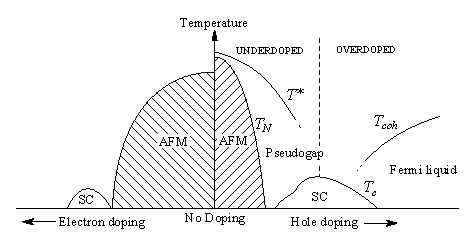
\includegraphics[scale=1.0]{Chapter-Introduction/Figures/ElecHolePhaseDiagram/ElecHolePhaseDiagram}
        \caption{A schematic phase diagram showing electron doped to the left and hole doped to the right. \ac{AFM} is the antiferromagnetic Mott insulating phase, SC is the superconducting phase. $T^*$, $T_N$, $T_c$ and $T_{\textrm{coh}}$ are the temperature scales for the pseudogap, \ac{AFM} state, superconductivity and coherent Fermi liquid phases respectively}
        \label{Fig:Intro:ElecHolePhaseDiagram}
    \end{center}
\end{figure}

\subsection{Mott insulating parent compound}

Starting at the middle of figure~\ref{Fig:Intro:ElecHolePhaseDiagram}, the parent compound materials at zero doping are thought to be Mott insulators i.e. the top most filled state on each lattice site contains one electron. In the conventional band picture this should be metallic since the bands are only partially filled, however when we consider a local picture of electrons, any movement of an electron to the neighbouring lattice site will cause an energetically costly double occupancy on one site and zero occupancy on another. This causes the electronic \ac{DOS} to become gapped around the Fermi surface and hence suppressed conduction. This is known as the Mott insulating state.

We find that the kinetic energy term is reduced when the ordering of the sites is antiferromagnetic since for any hopping to occur at all, the spins must be antialigned to avoid double occupancy of like spins. This region dominates the low doping portion of the phase diagram and remains antiferromagnetic until either the temperature is high enough to allow transitions from the Fermi energy to the states at the edge of the gap or the doping has introduced enough double occupancy electrons on lattice sites, which can move without the double occupancy energy cost, to overcome the insulating behaviour.

\subsection{Superconducting dome}

With increased doping, the antiferromagnetic state gives way to the superconducting dome at around $p=0.05$ which itself gives way to a Fermi liquid metallic state at a doping of around $p=0.3$. The maximum \Tc occurs at around $p=0.16$. Transitions from both the antiferromagnetic and the superconducting state are clearly second order thermodynamic with jumps in the heat capacity for example, however there are other regions in the phase diagram which are less well defined such as the pseudogap and the Fermi liquid crossover whose temperature scale can depend on the particular probe used and do not feature a clear order parameter.

\subsection{Coherent phase}

To the heavily overdoped side of the phase diagram, beyond the superconducting dome lies the coherent region where the system bears the hallmarks of a conventional metal. The implication is that correlations between electrons are sufficiently weak such that the mass enhanced quasiparticles of Landau's Fermi liquid theory are well defined, leading to conventional metal behaviour. A clear indication of this is a dominant $T^2$ term in the resistivity. Above this region we observe an anomalous additional contribution which has been modelled both with $T^2$ plus an additional linear term or by a $T^n$ term where $1 <= n <= 2$. This additional term has been observed in heavy Femrion materials and is often associated with proximity to a \ac{QCP}~\cite{Custers2003}.

\subsection{The pseudogap}

Above the antiferromagnetic region and the superconducting state is one of the most controversial regions of the phase diagram, the so called pseudogap phase. This is a region which was first demonstrated in 1989, just a few years after the discovery of the cuprate materials, by \ac{NMR} measurements performed at Bell labs~\cite{Warren1989}. A noticeable fall in the susceptibility occurred at a temperature significantly above $T_c$ which led to conclusion of possible spin pairing before the onset of bulk superconductivity\footnote{Cooper paired electrons in the singlet state have zero net spin hence they do not contribute to the susceptibility, whereas unpaired electrons do. Cooper pairing leads to a reduction in susceptibility, see for example neutron scattering plots.}. The question arose as to what the exact relation of the pseudogap is to the superconducting state --- is it a precursor state, from which superconductivity arises or is it a competing phase? --- and from a materials development point of view, to obtain higher $T_c$ should we be finding ways to suppress the crossover to the pseudogap state or encourage it?
\begin{figure}[htbp]
    \begin{center}
        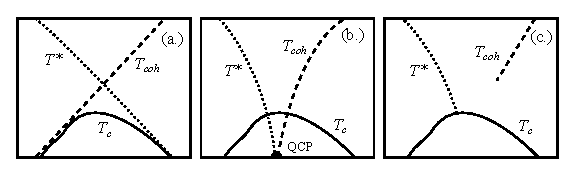
\includegraphics[scale=1.0]{Chapter-Introduction/Figures/PGScenarios/PGScenarios}
        \caption{Three scenarios proposed for the $T^*$ temperature scale behaviour. (a.) the pseudogap as the `precursor' state, (b.) as the `competing' state, (c.) and the `transition' scenario.}
        \label{Fig:Intro:PGScenario}
    \end{center}
\end{figure}
By finding where exactly the $T^*$ energy scale meets the superconducting dome, strong evidence can be found that supports one or the other scenario. However the problem lies in the type of probe used. Select spectroscopic measurements including \ac{STM}, \ac{ARPES} and Raman spectroscopy on materials of comparable $T_c$ values have found that the $T^*$ overreaches the superconducting dome entirely~\cite{Hufner2008}, meeting with the overdoped edge at $T=\unit{0}{\kelvin}$. This supports the precursor state theory illustrated in figure~\ref{Fig:Intro:PGScenario}~(a.) where $T^*$ and $T_{\textrm{coh}}$ cross to define a region which is below both temperature scales where the carrier are both coherent quasiparticles and paired leading to the superconducting condensate.

A second scenario is supported by measurements using bulk probes such as heat capacity, magnetic susceptibility and resistivity measurement have shown the $T^*$ energy scale drops into the top of the superconducting dome~\cite{Tallon2001}. This supports the scenario where the pseudogap is in competition with superconductivity for states at the Fermi surface. Once the pseudogap phase is suppressed, scattering from quantum fluctuations at zero temperature leads to the formation of the superconducting phase at a \ac{QCP} similar to that found in heavy fermion materials. This scenario is supported by the observation of linear scaling of the resistivity with temperature in the region above the superconducting dome which is a hallmark of proximity of a \ac{QCP}.
% Kondo is a competitive scenario which justified based on
% non-monotonicity of coherence as you move from the antinodes on the FS \cite{Kondo2009}

A third scenario is one where the pseudogap simply becomes the superconducting gap as it meets the top of the superconducting dome. However this scenario leaves hanging questions as to the roles of the pseudogap, $T_{\textrm{coh}}$ and other phenomena in the phase diagram which would need to be addressed theoretically. Moreover this picture is rendered less compelling by the observation in \ac{LSCO} of rapidly increasing, low temperature, normal state resistivity inside of the underdoped superconducting dome which implies the non-superconducting energy gap persists into this region.


\subsection{Previous work by the Bristol group}

Clearly lots of interesting physics is occurring in and around the superconducting dome and a solid understanding of this region is key to understanding the problem of high-$T_c$. Prof. N. Hussey has been involved in many efforts to shed light on the situation, of which, two key ones are highlighted here.

\subsubsection{Links between anisotropic scattering and $T_c$}

Simply measuring resistance along different axes gives an averaged scattering rate through all conduction paths and so to build a map of the angle dependent scattering rates, a different technique must be used. In \ac{ADMR} a strong persistent magnetic field is applied before resistance measurements are taken. The field serves two purposes; firstly, to suppress superconductivity so the normal state can be probed, secondly to confine the electrons to orbits perpendicular to the field. By detailed analysis of the change in resistance as the field is applied at various angles, a picture of the angle dependent scattering rate can be determined.

After performing measurements on samples of \ac{TL2201} with dopings ranging from strongly overdoped to slightly underdoped~\cite{Abdel-Jawad2006}, a trend emerged which is illustrated in figure~\ref{Fig:Intro:AnisotropyPhase}. 
\begin{figure}[htbp]
    \begin{center}
        \includegraphics[scale=0.9]{Chapter-Introduction/Figures/AnisotropyPhase/AnisotropyPhase}
        \caption{Schematic of how the scattering rate, $\Gamma$, the Fermi surface, $FS$, and the superconducting gap, $\Delta_g$ evolve with doping across the superconducting dome. Based on figure 1 in ref~\cite{Taillefer2006}. The dotted line in the scattering is the isotropic part.}
        \label{Fig:Intro:AnisotropyPhase}
    \end{center}
\end{figure}
Here the scattering rate within the $ab$-plane, $\Gamma$, was found to be composed of two terms; an isotropic term which remained constant with doping (dotted circle) and an anisotropic component which scaled with the superconducting gap, $\Delta_g$. Moreover it was found that the superconducting gap and the anisotropic scattering rate both shared the same shape, being `d-wave'. This further ties to \ac{ARPES} measurement which show that the on the underdoped side of the superconducting dome there is a pronounced change in the Fermi surface where at the antinodal points of $\Gamma$ (and $\Delta_G$) the spectral weight disappears~\cite{Norman2010} i.e. coherent particles are lost away from the regions of strong scattering.

%It changes from a single large hole band of volume $1+p$ to series of small regions of electron and hole Fermi surface of total volume $p$.

\subsubsection{T-Linear behaviour in the superconducting dome}

Previous high-field transport measurements on Sr doped \ac{LSCO}~\cite{Cooper2009} gave key insights into the nature of the T-linear term as it entered the superconducting term on the overdoped side. In particular it showed that the T-linear term did not funnel down to a point (figure~\ref{Fig:Intro:CooperTLinear}) as is typical of \ac{QCP} behaviour but instead spread out into the superconducting region. Intrigued as to this unexpected behaviour, we looked to repeat the measurements on \ac{BSCO} which can be doped far more widely without divergence in the resistivity so that we could then see how the T-linear term progressed on the underdoped side, where $T^*$ is undisputed.
\begin{figure}[htbp]
    \begin{center}
        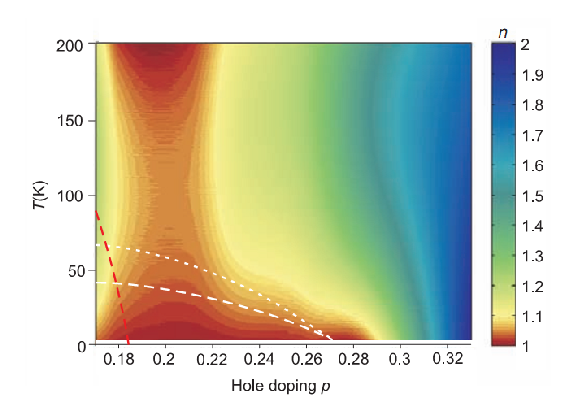
\includegraphics[scale=0.8]{Chapter-Introduction/Figures/CooperTLinear/CooperTLinear}
        \caption{Plot of the $T^n$ term in the fitted field suppressed normal state of Sr doped \ac{LSCO} showing the $T$-linear term extending throughout the superconducting dome and not to a single \ac{QCP}. Taken from Cooper \etal~\cite{Cooper2009}}
        \label{Fig:Intro:CooperTLinear}
    \end{center}
\end{figure}
Performing measurements which would shed light onto which of the scenarios shown in fig~\ref{Fig:Intro:PGScenario} is most likely to be correct formed the original motivation for the investigation of \ac{BSCO} through transport measurements. 

A second reason for the study of \ac{BSCO} in particular is that it's van-Hove singularity occurs at a different doping --- further from optimal doping --- than \ac{LSCO}. Should similar behaviour be found then we can confidently claim that the unusual \ac{QCP} behaviour is not due to proximity to the changeover in hole-like to electron-like Fermi surface and is likely universal to all cuprates. 

\ac{BSCO} also demonstrates transport behaviours which are consistent with other high-$T_c$ cuprate materials. For example, from \ac{MR} measurements it demonstrates a similar maximum in the underdoped $d\rho_{ab}/dT$ curve as underdoped YBCO~\cite{Ando1999}. On the overdoped side, \ac{BSCO} demonstrates a monotonic upward trend in $d\rho_{ab}/dT$ with increasing temperature similar to what has been observed in Tl$_{2201}$ and \ac{LSCO}~\cite{Ando1999}.

During the course of the investigations however, it became apparent that even with field strengths of up to \unit{60}{\tesla} in pulsed fields, the upper critical field, $H_{\textrm{c2}}$ of many of the sample at key temperatures could not be reached. However, field strengths were generally strong enough to recover $B$-Linear behaviour in the Hall component.

Previous Hall measurements have been performed on \ac{BSCO} by Ando \etal~\cite{Ando1999, Ando2000} which are shown for comparison in the results section. However these results do not go to low temperatures, being restricted by the onset of superconductivity. Our own results used high field measurements at \ac{LNCMI} and \ac{HFML} to suppress superconductivity and examine the low temperature regions in detail. Moreover our samples are focused on the overdoped region which complements the underdoped data set presented in the Ando papers.

% Motivation

% Lograithmic divergence of scattering rate observed in cuprates which
% begins at critical doping and increases as become more underdoped.
% However common factor of cuprates (Y123, Tl2201, LSCO) is a change of
% Fermi surface (in LSCO at least) from hole to electron leading to a
% van Hove singularity(?) which occurs similar to hwere would expect the
% insulating crossover. This does not occur in BSCO however until
% around p=0.2\cite{Hashimoto2008}. If the \alpha^2 term takes off
% earlier for BSCO\cite{Hussey2011a} is good
% evidence that is due to the proximity to van Hove rather  than Moot
% insulator transition.\cite{Ono2000}


% \section{Mott physics}

% The Hubbard model takes the relatively simple and solvable tight-binding model and introduces an Anderson term which raises the energy for double occupancy by an amount $U$, known as the `Hubbard U'. This simple change deeply enriches the physics with one of the outcomes being the existance of the Mott insulating state which occurs when each lattice site is half filled with a single electron. The energy cost for an electron to hop to an adjacent site is so high that it locks the electrons in place, preventing effective conduction. Introducing holes (or electrons) allows once again hopping to take place and the eigenstates are no longer entireley localised.




\section{Fermi surface nesting as a pairing mechanism}

The charge carrier in a superconducting condensate is a Cooper pair - a quasi-particle comprising of a bound state of two electrons or two holes with opposite spin and momentum. Evidence for this configuration arises as a natural result of the Ginzberg-Landau model which, when applied to a superconducting system, gives the charge of the quasi-particle carriers as $2e$, where $e$ is the charge of an electron. Given that due to their like charges two free electrons repel, it is natural to ask what could overcome the electromagnetic force to cause these electrons to remain bound in this quasi-particle state.

Bardeen, Cooper and Schreiffer established much of the theoretical basis --- from which the Ginzberg--Landau model can be derived --- in \textit{BCS theory} (named after the authors) and within the framework of BCS theory, wrote a 1957 paper\cite{Bardeen1957} detailed a pairing mechanism known as the \textit{BCS model} which would explain how these electron remained bound together. The model is based around the concept of phonons scattering off ions which well suited the superconducting materials known at the time. Phenomenologically, the mechanism of attraction is straightforward. Electrons moving through a crystal lattice attract ions on the lattice sites. These heavy ions respond slowly and are drawn in \textit{behind} the electron. This has the effect of both screening the negative electron charge as well as providing an attractive positive potential for any electron following the original electron. The net effect is the leading electron draws the following electron in its wake, thus coupling them with one another. The wavelike distortion of the ions in the lattice can be considered as a phonon, and the interaction between the electrons and the lattice can be modelled as electron--phonon--electron scattering.

The BCS model on top of BCS theory accurately describes what we now know as \textit{conventional superconductivity}, that is pairing which forms a spin-singlet state ($S=0$) and which has zero orbital angular momentum ($L=0$). It was not until the discovery of superfluidity\footnote{Superfluidity and superconductivity share much of the same physics although rather than electrons or holes pairing, molecules pair instead. Parallels betwen the two are discussed in ref.\cite{Annett2010}} in $^3$He in 1972\cite{Osheroff1972} that it became apparent that there may exist forms of pairing that resulted in spin-triplet pairing state ($S=1$) with $L>0$. This was later confirmed when superconducting analogues were found in the form of heavy Fermion materials. What really spurred the explosion in interest though was the 1986 discovery by Bednorz and M\"uller\cite{Bednorz} of high transition temperature (\Tc) superconductivity in the cuprates and, more recently, the `pnictides' by Kamihara et al.\cite{Kamihara2008}. The cuprate class of materials that Bednorz and M\"uller found to be superconducting have \Tc~s far in excess of any previously known superconducting materials and although the BCS model phonon pairing may play a part, the predominant pairing mechanism in the \highTc materials is likely to be something else entirely.

\subsection{The case against conventional superconductivity in \highTc}

There is a great deal of evidence in the literature for non-BCS model pairing in the \highTc and heavy Fermion materials. Although the pairing wavefunction cannot be measured directly with current techniques, experiments indirectly infer \textit{unconventional} i.e. non s-wave, BCS-model, characteristics. For example, analysis on penetration depth measurements of YBa$_2$Cu$_3$O$_{7-\delta}$ show power law behaviour\cite{Annett1991}, indicating that there exists states within the momentum averaged gap. SQUID measurements and Josephson tunneling experiments on the same material have confirmed alternating phase of the condensate wavefunction which points strongly to \DxTwoyTwo--wave symmetry\cite{VanHarlingen1994} (see also refs. therein). As for other cuprate materials, specific heat measurements on \BSCO\cite{Wang2011}, as well as peentration depth measurements on LSCO\cite{Froehlich1996} have also proved consistant with $d$-wave pairing. 

More evidence against conventional superconductivity include the unusual normal state (i.e. non-superconducting) state properties of the cuprates and heavy Fermion materials. The BCS model is grounded in Landau Fermi liquid theory which models interacting itinerent electrons with quasiparticles of heavier effective mass than ordinary electrons and holes. A hallmark of Fermi liquid behaviour is a $T^2$ dependence of the resistance, however experiments on the cuprate La$_{2-x}$Sr$_{x}$CuO$_4$\cite{Cooper2009} and a heavy Fermion material\cite{Custers2003} have demonstrated fractional power law behaviour, $T^\gamma$ where $1 < \gamma < 2$, at temepratures above the superconducting transition. Given that the Fermi liquid model breaks down in these examples, it follows that the BCS-model also is likely on shaky ground for these materials.

There are several arguments against phonons as the sole pairing mechanism in the pnictide case, Boeri et al.\cite{Boeri2008} and Mazin et al.\cite{Mazin2008} present calculations showing that the magnitude of the phonon pairing strength is not adequate for the high \Tc values attained in LaAsOF, Haule et al.\cite{Haule2008} note in the same material that the gradient of the density of states (DOS) at the Fermi level is such that you would expect an increase in DOS and hence \Tc with hole doping if the BCS model held, however the reverse is true. Non Fermi-liquid behaviour was demonstrated in the \BaFePAs series\cite{Jiang2009,Kasahara2010} and evidence for nodes in the gap function have been found in LaFePO\cite{Fletcher2009} and the \BaFePAs series\cite{Zhang2011,Yamashita2011a,Suzuki2011} although not in % TODO

It is interesting to note that Unlike the cuprates which universally show a \DxTwoyTwo gap symmetry, the pnictide materials are note all alike. As a result, it may prove that the nature of the supercondcutivity may not be universal amongst the pnictide materials. Irrespective of this, there is no evidence for BCS model pairing in the pnictide materials and in many cases, BCS pairing has been shown to be insufficient.


\subsection{Spin-fluctuations}

Soon after the discovery of the pnictide materials, a possible pairing mechanism was proposed based on spin density wave fluctuations. The original paper suggested a $s_{\pm}$ gap symmetry which does not feature any nodes however 

\subsection{Pnictides}

Some arguments against the BCS theory of pairing \cite{Haule2008,Yndurain2009,Mazin2008} based on arguments of 

FS nesting not the only cause of spin-fluctuations, also can be caused by frustrated superexchange for example % TODO

Spin fluctuations mediate a repulsive interaction between Cooper pair candidates.

The anisotropic BCS equations specify that repulsive coupling between carriers can be pairing provided the order parameter changes sign over the coupling vector.


There are several proposed mechanisms presently on offer including charge fluctuations resulting in large ion polarisation \cite{Berciu2009}, however this was contested by Mazin and Schmalian\cite{Mazin2009}.


Of these theories, the one with arguably the most traction at present is that of spin-fluctuation mediated pairing. 

TODO: What actually is the cause of the attraction in the nesting picture? ... Spin fluctuation intereaction in real space is approximately propoprtional to the dipole interaction $V=-\mu . \mu \chi(r)$\cite{Bergemann2003} 



Strong correlations - the interaction energy is much greater than the kinetic energy for the states
When correlations present, Cooper pairs are assumed to be pairs of Landau quasiparticles


\subsection{Susceptibility}
    \label{Sec:Intro:NestingSusceptibility}

A commonly used measure of the nesting condition is the Lindhard susceptibility function. This is often quoted as,
\begin{equation}
\chi_0(\vec{q}, \omega) = \lim_{\eta \to 0} \sum_{\vec{k}}\sum_{l,l\prime}\frac{f(\epsilon_{\vec{k}+\vec{q},l\prime}) - f(\epsilon_{\vec{k},l})}{\epsilon_{\vec{k}+\vec{q},l\prime} - \epsilon{\vec{k},l} - \hbar\omega - i\eta}|\langle \vec{k}+\vec{q},l\prime \mid  V \mid \vec{k},l \rangle|^2
\label{Eqn:Intro:Lindhard}
\end{equation}
respectively. The numerator term contains two Fermi functions ($f(\epsilon) = 1/(\exp{\frac{\epsilon - \epsilon_F}{k_B T}} + 1)$) where $\epsilon$ and $\epsilon_F$ are the state energy and the Fermi energy respectively and $k_BT$ is the usual Boltzman energy conversion factor. These Fermi functions ensure that the susceptibilty is finite for states which scatter across the Fermi energy and zero if they do not. They also smear the calculations as a function of temperature. The final term in the denominator is an artefact of the adiabatic approximation used to calculate the perturbation. The completed approximation takes the limit of $\eta \to 0$ which results in an expression for the imaginary part of Lindhard susceptibility, $\mathcal{Im}(\chi_0) \propto \delta(\epsilon_{\vec{k}+\vec{q},l\prime} - \epsilon{\vec{k},l} - \hbar\omega)$ which, in a continuous calculation, results in resonances at excitations which match the difference in energies between states. However, in this thesis, the energy dispersions used to determine nesting conditions are not continuous and instead are based on discrete energies obtained from DFT calculations. As such $\eta$ will have to remain finite in order to broaden the delta function into a Lorentzian with width comparable to the energy differences between the discrete points -- the net result of this will be loss of some fine structure. The third term in the denominator corresponds to the excitation energy of the perturbing field with $\omega$ corresponding to the temporal frequency of the field. The first sum in the Lindhard function is over all $\vec{k}$ states in the first Brillouin zone. The DFT calculations do not provide values for all $\vec{k}$ states, instead a fairly coarse mesh evenly distributed over the Brillouin zone is used. The second sum combines each energy band. In practice only bands that lie close (within the adiabatic or temeprature broadening) to the Fermi energy need to be included in the calculations.

Peaks in this function correspond to scattering of states which cross the Fermi energy yet remain close to the Fermi energy.  We can derive this function by modelling an oscillatory perturbing field on a system. To solve to get an expression for the second order perturbation, we make the adiabatic limit approximation (i.e. the perturbing potential is gradually increase from zero at $t=\infty$ to $v$ at $t=0$).

The real and imaginary parts of equation \ref{Eqn:Intro:Lindhard} are,
\begin{align}
\chi_0(\vec{q}, \omega)\prime &= \lim_{\eta \to 0} \sum_{\vec{k}}\sum_{l, l\prime}\frac{(\epsilon_{\vec{k}+\vec{q},l\prime} - \epsilon{\vec{k},l} - \hbar\omega) f(\epsilon_{\vec{k}+\vec{q},l\prime}) - f(\epsilon_{\vec{k},l})}{(\epsilon_{\vec{k}+\vec{q},l\prime} - \epsilon{\vec{k},l} - \hbar\omega)^2 + \eta^2}|\langle \vec{k}+\vec{q},l\prime \mid  V \mid \vec{k},l \rangle|^2 \\
\chi_0(\vec{q}, \omega)\prime\prime &= \lim_{\eta \to 0} \sum_{\vec{k}}\sum_{l, l\prime}\frac{-\delta f(\epsilon_{\vec{k}+\vec{q},l\prime}) - f(\epsilon_{\vec{k},l})}{(\epsilon_{\vec{k}+\vec{q},l\prime} - \epsilon{\vec{k},l} - \hbar\omega)^2 + \eta^2}|\langle \vec{k}+\vec{q},l\prime \mid  V \mid \vec{k},l \rangle|^2 \\
\end{align}
respectively.

Although knowledge of the susceptibility is useful to model, for example, neutron scattering measurements, for our purposes we will use it to demonstrate the strength of particular nesting vectors in our example materials. For this reason we make the assumption that the transition matrix elements are unity. This assumption greatly simplifies the calculations at the cost of some structure and as such should be borne in mind that the results are somewhat broad and qualitative.


TODO: How does susceptibility tie in with nesting?
TODO: Lindhard susceptibility is a time dependent perturbation in the adiabatic limit to what? Adiabatic limit is where the pertubation time-frame is slow c.f. the unperturbed time-frame 
TODO: imaginary factor corresponds to the decay rate of the state
TODO: energy(susceptibility) is broadened by the decay rate




% The Stoner condition of $\mathcal{N}_0 I > 1$ -- where $\mathcal{N}_0$ is the density of states at the Fermi energy and $I$ is the molecular field constant, that scales the magnetism given a field -- indicates an energy instability\cite{Kubler2000}



\section{The pseudogap vs. the coherent state}

The phase diagram for the cuprates, when hole doping is the tuning parameter, appears to be universal, however, at the time of writing, is somehwhat more complicated than that of a typical pnictide\footnote{In general there is more variation in the phase diagram amongst pnictide materials, however there are less features in these diagrams when compared to the cuprates}. With reference to the schematic cuprate phase diagram shown in figure~\ref{Fig:Intro:UniversalCupratePhaseDiagram} we see several temperature scales that may or may not be of interest to the underlying causes of \highTc superconductivity.
\begin{figure}[htbp]
    \begin{center}
        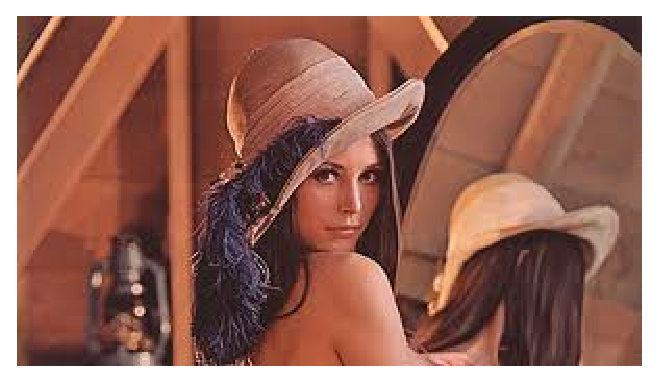
\includegraphics[scale=0.7]{Misc/TODO}
        \caption{A schematic phase diagram of a series of hole-doped cuprates}
        \label{Fig:Intro:UniversalCupratePhaseDiagram}
    \end{center}
\end{figure}
From the standpoint of conventional superconductivity, the first striking feature is the proximity of an antiferromagnetic phase to the superconducting region. Even without actual temperature labels, it becomes clear that if this was a phonon mediated superconductor, the pairing must be strong in order to overcome the strong spin-density wave scattering that results in the anitferromagnetic state.

Another interesting region, one that is not present in the pnictides, is that below the $T^*$ temperature scale on the underdoped side of the superconducting dome. In this region, an energy gap opens up in the excitation spectra but without any sign of the Meissner effect. This region is known as the \textit{pseudogap}. Some aspects of the pseudogap lead us to believe that it is closely related to the superconducting gap such as the fact that it shares the gap symmetry and is of a similar magnitude, and there have been proposals that the pseudogap is a precursor state to superconductivity TODO. However research involving the Bristol group has shown evidence that phase fluctuations rather than the pseudogap in particular are the neceesary precursors for the cuprate superconducting condition\cite{Rourke2011}.

\subsection{Anisotropic scattering}





\section{Cuprate doping determination}



